\documentclass[11]{beamer}
\usepackage{hyperref}
\usepackage{graphicx} % Allows including images
\usepackage{booktabs} % Allows the use of \toprule, \midrule and \bottomrule in tables
\usepackage{pgfgantt}
\usepackage[portuguese]{babel}
\usepackage{ragged2e} % Justificar texto

% Definições do tema
\usetheme{copenhagen} % Pode ajustar para outro tema se necessário
\usecolortheme{default}
\setbeamertemplate{navigation symbols}{} % Remove os símbolos de navegação
\setbeamertemplate{headline}{} % Remove o cabeçalho

% Informação da capa:
\title{Ferramenta para Geração de Horários de Cursos com Restrições}
\subtitle{Apresentação do Relatório de Desenvolvimento do Trabalho}

\author[Ricardo Ramos]{Ricardo Alexandre Alves Ramos}

\institute[ISEL]{Instituto Superior de Engenharia de Lisboa}

%\date{Março 01, 2025}
\date{\today}

\institute{
    Instituto Superior de Engenharia de Lisboa \\ 
    Departamento de Engenharia Eletrónica e de Telecomunicações e Computadores \\ 
    Mestrado em Engenharia Informática e de Computadores
}

\begin{document}
    %----------------------------------------------------------------------------------------
    %    PRESENTATION SLIDES
    %----------------------------------------------------------------------------------------

    % Slide de título
    \begin{frame}
        \begin{center}
            \begin{beamercolorbox}[rounded=true, shadow=true, sep=10pt, center, wd=\linewidth]{title}
                \color{white} \usebeamerfont{title} \textbf{\inserttitle} \\
                \usebeamerfont{subtitle} \insertsubtitle
            \end{beamercolorbox}
            
            \vspace{1em}
            {\usebeamerfont{author} \insertauthor}

            \vspace{1em}
            {\footnotesize
            Orientadores: Prof. Doutor Nuno Miguel da Costa de Sousa Leite \\
            \vspace{-1mm}\hspace{-.5cm}Prof. Doutor Artur Jorge Ferreira}
            
            \vspace{1em}
            {\usebeamerfont{institute} \insertinstitute}
            
            \vspace{2em}
            {\usebeamerfont{date} \insertdate}

            \vspace{-1.5em}\hspace{7.5cm}
            
\includegraphics[width=2.5cm]{img/logoisel.png}
        \end{center}
    \end{frame}

    \begin{frame}{Índice}
        \tableofcontents
    \end{frame}

    %------------------------------------------------
    \section{Introdução}
    %------------------------------------------------

    \begin{frame}{Problemas de Agendamento}
        \justifying
        Os problemas de agendamento são problemas de otimização combinatória muito complexos. Estes problemas existem em várias áreas como: Ensino, Medicina, Transporte, Logística, entre outros.

        \vspace{.5em}
        Na área de ensino, os problemas de agendamento podem ser abordados por meio de duas formulações:
        
        \vspace{.5em}
        \begin{itemize}
            \item Agendamento de Disciplinas Baseado no Currículo (CB-CTT)
            \item Agendamento de Disciplinas Após Inscrição (PE-CTT)
        \end{itemize}
    \end{frame}

    \begin{frame}
        \justifying
        Os problemas de agendamento escolar podem ainda ser divididos em três categorias:

        \vspace{.5em}
        \begin{itemize}
            \item Agendamento Escolar (\textit{School Timetabling})
            \item Agendamento de Cursos Universitários (\textit{Course Timetabling})
            \item Agendamento de Exames (\textit{Examination Timetabling})
        \end{itemize}
        \vspace{.5em}

        Este projeto terá um foco na categoria de Agendamento de Cursos Universitários com a formulação Agendamento de Disciplinas Baseado no Currículo.
    \end{frame}

    %------------------------------------------------
    \section{Estado da Arte}
    %------------------------------------------------

    \subsection{Algoritmos tipicamente utilizados}

    \begin{frame}{Algoritmos tipicamente utilizados}
        \justifying
        Algoritmos tipicamente utilizados na resolução de problemas de agendamento de cursos universitários. 
        \begin{itemize}
            \item Coloração de Grafos (\textit{Graph Coloring})
            \item Coloração de Arestas (\textit{Edge Coloring})
            \item Programação Inteira (\textit{Integer Programming})
            \item Procura Tabu (\textit{Tabu Search})
            \item Têmpera Simulada (\textit{Simulated Annealing})
        \end{itemize}

        Nos últimos anos, tem-se verificado um aumento na utilização de algoritmos híbridos para a resolução deste tipo de problemas. Estes algoritmos visam combinar características específicas de diferentes abordagens, aumentando o seu desempenho e eficiência.
    \end{frame}

    \subsection{Empresa \textit{Bullet Solutions}}

    \begin{frame}{Empresa \textit{Bullet Solutions}}
        \justifying
        A empresa \textit{Bullet Solutions} é uma empresa tecnológica especializada no desenvolvimento de soluções para otimização de recursos e gestão de horários.

        O projeto será desenvolvido com o objetivo de oferecer uma alternativa competitiva à aplicação disponibilizada pela \textit{Bullet Solutions}, que é atualmente utilizada no ISEL.
    \end{frame}

    \begin{frame}
        \justifying
        Solução disponibilizada pela \textit{Bullet Solutions}:
        \begin{center}
            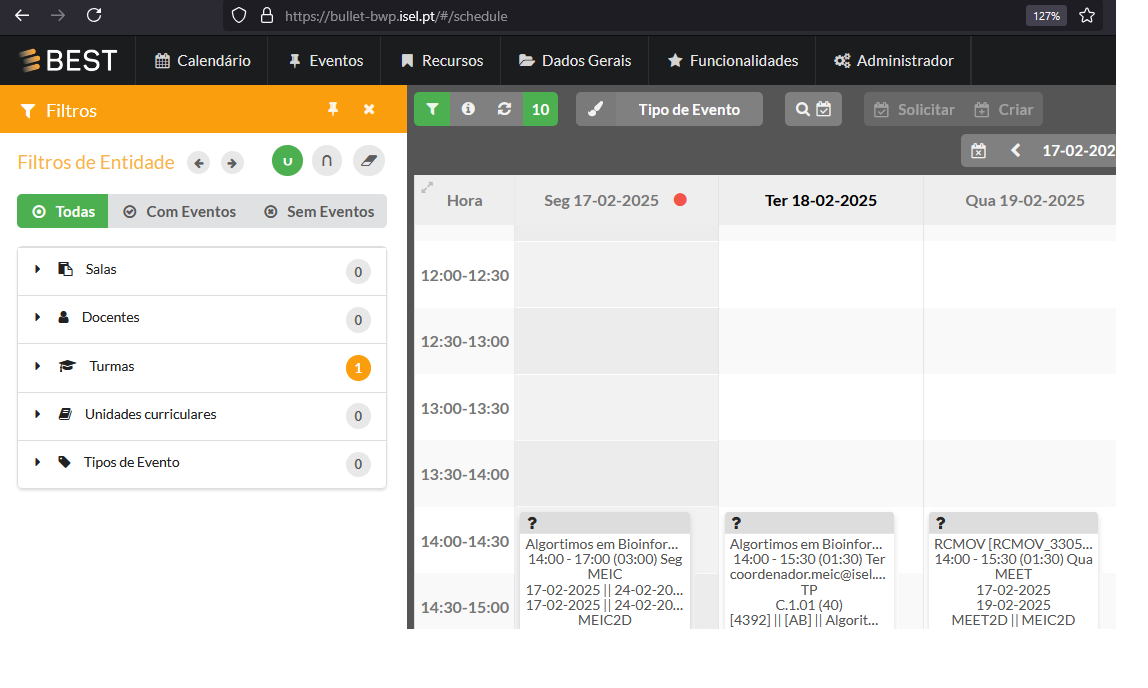
\includegraphics[width=10cm]{img/exemplo-bullet-solutions-software.png}
        \end{center}
    \end{frame}

    %------------------------------------------------
    \section{Trabalho Realizado}
    %------------------------------------------------

    \subsection{Diagrama de blocos}

    \begin{frame}
        Diagrama de blocos:
        \begin{center}
            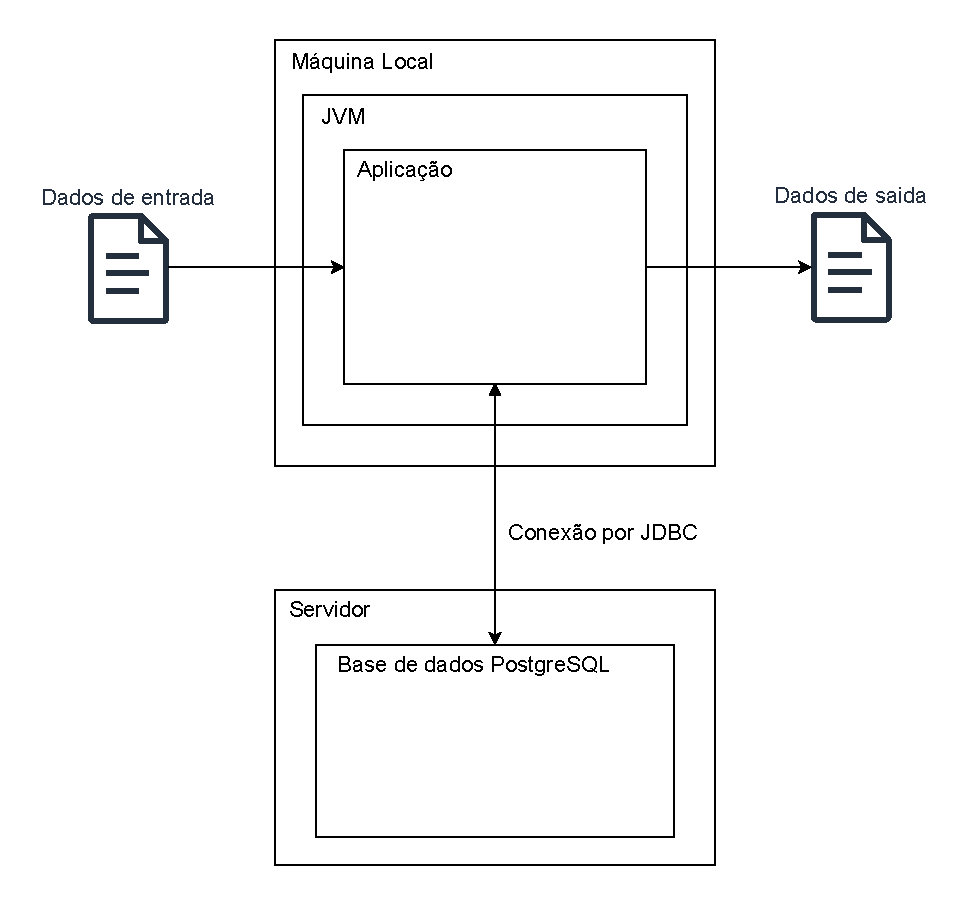
\includegraphics[width=.85\linewidth]{img/diagrama-blocos.pdf}
        \end{center}
    \end{frame}

    \subsection{Tarefas realizadas}

    \begin{frame}
        \justifying
        Tarefas realizadas:
        \begin{itemize}
            \item Definição do contexto e objetivos do projeto
            \item Análise das técnicas propostas na literatura
            \item Definição do diagrama de blocos
            \item Definição dos requisitos funcionais e não funcionais
            \item Análise detalhada do padrão proposto
            \item Definição dos casos de utilização
            \item Definição das restrições dos horários
        \end{itemize}
    \end{frame}

    %------------------------------------------------
    \section{Trabalho Futuro}
    %------------------------------------------------

    \subsection{Diagrama de Gantt}

    \begin{frame}{Diagrama de Gantt}
        \justifying
        \begin{figure}
            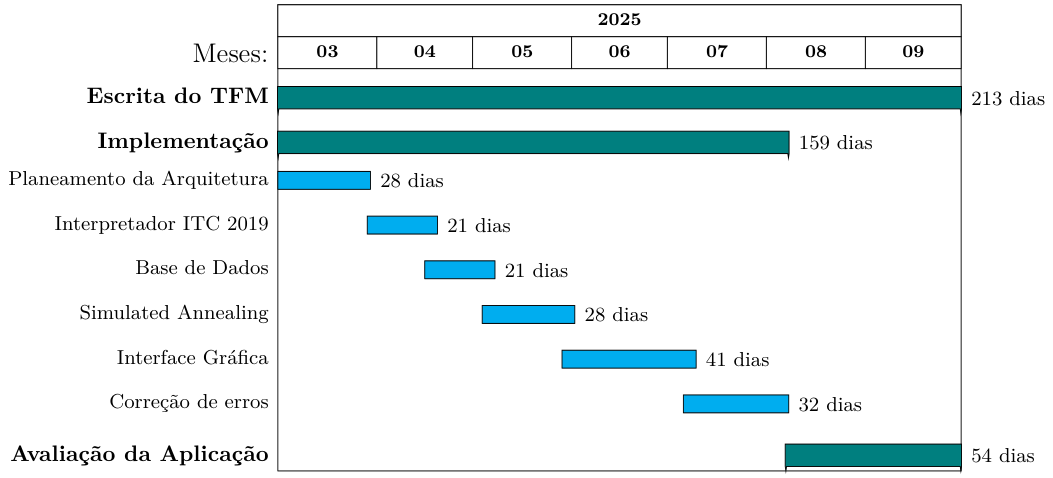
\includegraphics[width=\linewidth]{img/Diagrama-Gantt.png}
            %\caption{Diagrama de Gantt}
        \end{figure}
    \end{frame}

    \subsection{Tarefas Principais}

    \begin{frame}{Tarefas Principais}
        \justifying
        \begin{enumerate}
            \item Implementação de um sistema de importação de dados XML de acordo com o padrão da ITC 2019
            \item Disponibilizar a importação manual dos dados
            \item Apresentação de erros ao utilizador caso ocorra alguma falha no funcionamento do sistema
            \item Apresentação de conflitos no caso de impossibilidade de criação de horários
            \item Criação de interface gráfica simples e fácil de utilizar
            \item Permitir ajustes manuais aos horários gerados
            \item Implementação e otimização dos parâmetros do algoritmo SA
            \item Implementação de base de dados para a persistência dos dados da aplicação
            \item Apresentação de \textit{feedback} visual durante o processo de geração de horários
        \end{enumerate}
    \end{frame}

    \subsection{Tarefas Secundárias}

    \begin{frame}{Tarefas Secundárias}
        \justifying
        \begin{enumerate}
            \item Definição de manchas de disponibilidade através da interface gráfica
            \item Definição de períodos para aulas partilhadas através da interface gráfica
            \item Criação de \textit{logs} detalhados do funcionamento do sistema
            \item Congelamento de salas e/ou professores no momento de geração de horários
        \end{enumerate}
    \end{frame}

    %----------------------------------------------------------------------------------------

\end{document}